\documentclass[12pt]{article}
\usepackage[a4paper, margin=2.5cm]{geometry}
\usepackage{setspace}
\onehalfspacing
\usepackage{graphicx}
\usepackage{amsmath, amssymb}
\usepackage{booktabs}
\usepackage{caption}
\usepackage{float}
\usepackage{hyperref}
\usepackage{pgfplots}
\usetikzlibrary{intersections, patterns, decorations.markings, calc}

\title{Econometrics II -- Assignment 1:\\
Forecasting Economic Growth and Growth-at-Risk}
\date{Spring 2026}

\begin{document}

\maketitle

% ─────────────────────────────────────────────────────────────────────────────
\section{Introduction}
% ─────────────────────────────────────────────────────────────────────────────
% [1] State the main question: propose a univariate model for US GDP growth,
%     produce one-step-ahead forecasts, and estimate Growth-at-Risk (GaR).
% [2] Motivate: relevance for policy and central banking (cite Adrian et al. 2019).
% [3] State the econometric approach: AR(p) / ARMA(p,q) class, estimated by
%     OLS / ML on 1990Q1–2009Q4, evaluated on 2010Q1–2024Q4.
% [4] Headline result: brief statement of preferred model and key forecast / GaR finding.


% ─────────────────────────────────────────────────────────────────────────────
\section{Description of the Data}
% ─────────────────────────────────────────────────────────────────────────────
% [1] Source: U.S. Real GDP (GDPC1) from the FRED Database, quarterly, 1990Q1–2024Q4.
% [2] Variable: y_t = log(GDPC1_t) - log(GDPC1_{t-4}), yearly growth rate.
% [3] Figure 1: full-sample time-series plot of y_t (evaluation period shaded).
% [4] Comment: apparent stationarity (no deterministic trend, bounded variance);
%     note COVID-19 outlier in 2020; motivate model class.

\begin{figure}[H]
    \centering
    % 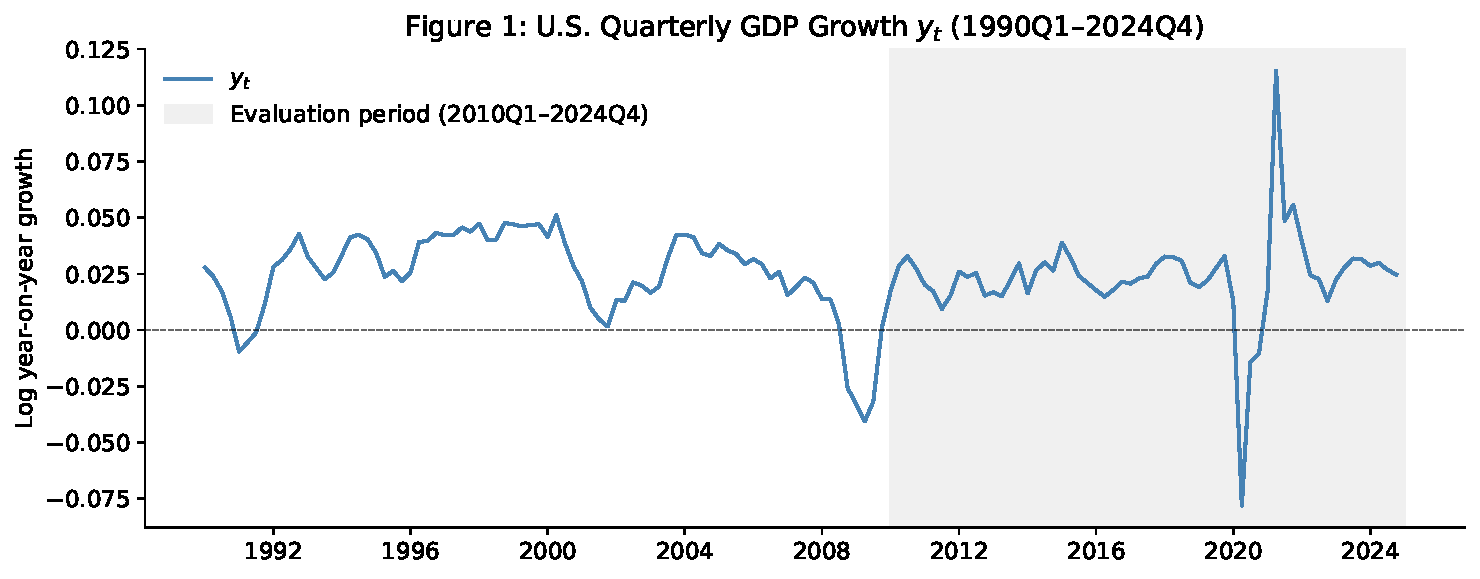
\includegraphics[width=\textwidth]{figures/fig1_gdp_growth.pdf}
    \caption{U.S. quarterly GDP growth $y_t$, 1990Q1--2024Q4.
             Shaded region indicates the out-of-sample evaluation period (2010Q1--2024Q4).}
    \label{fig:gdp_growth}
\end{figure}


% ─────────────────────────────────────────────────────────────────────────────
\section{Econometric Theory}
% ─────────────────────────────────────────────────────────────────────────────

\subsection{The ARMA Model}
% [1] Define the ARMA(p,q) model:
%       y_t = delta + phi_1 y_{t-1} + ... + phi_p y_{t-p}
%             + eps_t + theta_1 eps_{t-1} + ... + theta_q eps_{t-q}
% [2] State assumptions: eps_t ~ i.i.d. N(0, sigma^2); stationarity condition
%     (roots of AR polynomial outside unit circle).
% [3] Interpret delta as the unconditional mean (mu = delta / (1 - phi_1 - ... - phi_p)).

\subsection{Estimation}
% [1] AR(p): OLS estimator -- derive the estimating equation; state consistency
%     and asymptotic normality conditions (stationarity + ergodicity).
% [2] ARMA(p,q): Gaussian MLE -- state the log-likelihood; note OLS is a special case.
% [3] Model selection: AIC = -2 log L + 2k; BIC = -2 log L + k log T.
%     Prefer BIC for parsimony; also describe general-to-specific strategy.

\subsection{Forecasting}
% [1] One-step-ahead conditional mean:
%       E[y_{T+k} | I_{T+k-1}] = delta + phi_1 y_{T+k-1} + ... + theta_1 eps_{T+k-1} + ...
% [2] Recursive residual updates for ARMA component (reference forecasting_with_ARMA.tex).
% [3] Forecast error: e_{T+k} = y_{T+k} - yhat_{T+k}.
% [4] Diebold-Mariano test: H0: equal mean squared forecast error vs naive benchmark.

\subsection{Growth-at-Risk}
% [1] Define GaR: P(y_t <= GaR^alpha_t | I_{t-1}) = alpha.
% [2] Under Gaussian errors: GaR^alpha_t = mu_t + sigma * Phi^{-1}(alpha).
% [3] Evaluation: hit_t; violation rate p-hat; t-test H0: E[hit_t] = alpha.
% [4] Tick loss function T_alpha(y_t, GaR^alpha_t) = (alpha - hit_t)(y_t - GaR^alpha_t).


% ─────────────────────────────────────────────────────────────────────────────
\section{Empirical Analysis}
% ─────────────────────────────────────────────────────────────────────────────

\subsection{Model Selection}
% [1] Figure 2: ACF and PACF of y_t on training sample -- motivate AR vs ARMA.
% [2] Table 1: AIC, BIC, sigma-hat, Ljung-Box p-value for AR(1)--AR(4) and ARMA(1,1).
% [3] Justify preferred model.

\begin{figure}[H]
    \centering
    % 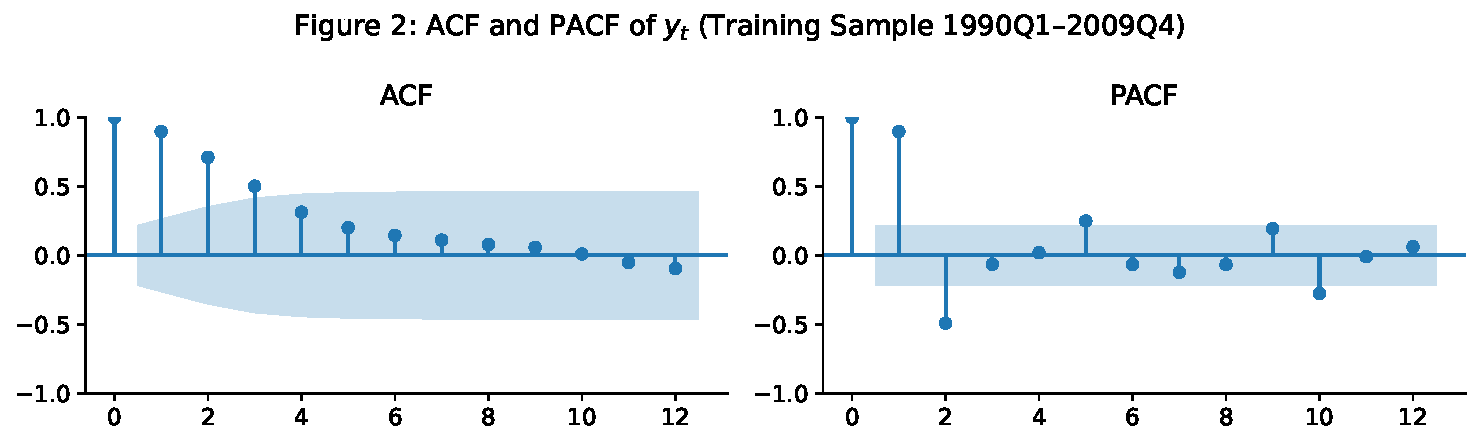
\includegraphics[width=\textwidth]{figures/fig2_acf_pacf.pdf}
    \caption{Sample ACF and PACF of $y_t$, training sample 1990Q1--2009Q4.
             Dashed lines indicate 95\% confidence bands.}
    \label{fig:acf_pacf}
\end{figure}

\begin{table}[H]
    \centering
    \caption{Model comparison: information criteria and diagnostics (training sample).}
    \label{tab:model_selection}
    % \begin{table}[H]
  \centering
  \caption{Model comparison: AIC, BIC, $\hat{{\sigma}}$, and Ljung-Box p-value (training sample 1990Q1--2009Q4).}
  \label{tab:model_selection}
  \begin{tabular}{lrrrr}
  \toprule
  Model & AIC & BIC & σ̂ & LB p-val (lag 8) \\
  \midrule
  AR(1) & -535.78 & -528.64 & 0.01 & 0.00 \\
  AR(2) & -551.86 & -542.33 & 0.01 & 0.14 \\
  AR(3) & -552.15 & -540.24 & 0.01 & 0.24 \\
  AR(4) & -550.23 & -535.94 & 0.01 & 0.28 \\
  ARMA(1,1) & -546.13 & -536.60 & 0.01 & 0.12 \\
  \bottomrule
  \end{tabular}
\end{table}

\end{table}

\subsection{Misspecification Testing}
% [1] Ljung-Box test for residual autocorrelation at lags 4 and 8.
%     H0: no autocorrelation up to lag m.
% [2] Jarque-Bera test for normality.
%     H0: residuals are normally distributed.
% [3] ARCH-LM test for conditional heteroskedasticity.
%     H0: no ARCH effects.
% [4] Discuss implications of any violations for inference validity.

\subsection{Preferred Model: Estimates and Interpretation}
% Table 2: coefficient estimates, standard errors, t-statistics, p-values.
% Interpret magnitude and significance of AR/MA coefficients.
% State estimated sigma-hat used for GaR.

\begin{table}[H]
    \centering
    \caption{Estimation results for the preferred model (training sample 1990Q1--2009Q4).}
    \label{tab:estimates}
    % \begin{table}[H]
  \centering
  \caption{Estimation results for the AR(2) model (training sample 1990Q1--2009Q4).}
  \label{tab:estimates}
  \begin{tabular}{lrrrr}
  \toprule
   & Coefficient & Std. Error & t-stat & p-value \\
  \midrule
  const & 0.0262 & 0.0060 & 4.3455 & 0.0000 \\
  ar.L1 & 1.3587 & 0.1235 & 11.0055 & 0.0000 \\
  ar.L2 & -0.5118 & 0.1241 & -4.1237 & 0.0000 \\
  sigma2 & 0.0001 & 0.0000 & 6.5740 & 0.0000 \\
  \bottomrule
  \end{tabular}
\end{table}

\end{table}

\subsection{Forecast Evaluation}
% [1] Figure 3: y_t, model forecast, naive forecast (evaluation period 2010Q1--2024Q4).
% [2] Table 3: RMSE (model vs naive), DM test statistic and p-value.
% [3] Interpret: does the AR model outperform the naive benchmark?

\begin{figure}[H]
    \centering
    % 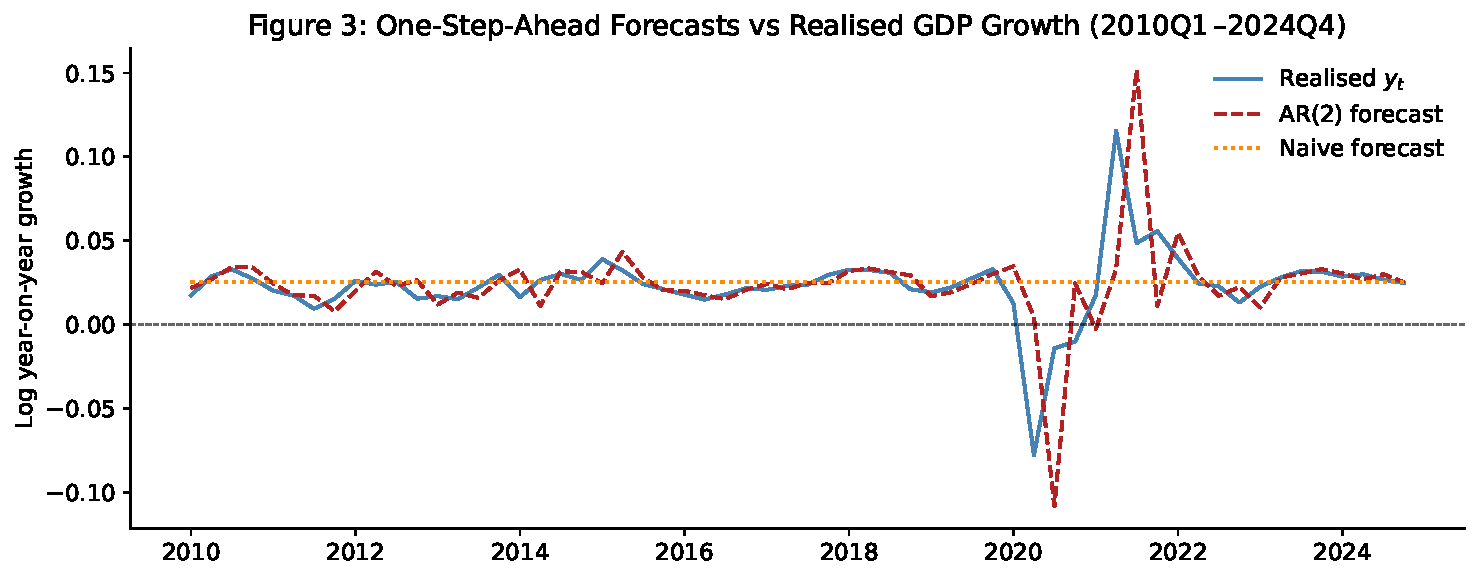
\includegraphics[width=\textwidth]{figures/fig3_forecasts.pdf}
    \caption{Out-of-sample forecasts vs realised GDP growth, 2010Q1--2024Q4.}
    \label{fig:forecasts}
\end{figure}

\begin{table}[H]
    \centering
    \caption{Forecast evaluation: RMSE and Diebold-Mariano test.}
    \label{tab:forecast_eval}
    % \begin{table}[H]
  \centering
  \caption{Forecast evaluation: RMSE and Diebold-Mariano test (2010Q1--2024Q4).}
  \label{tab:forecast_eval}
  \begin{tabular}{lrrr}
  \toprule
  Model & RMSE & DM statistic & DM p-value \\
  \midrule
  AR(2) & 0.0256 & 1.0450 & 0.2960 \\
  Naive & 0.0206 & — & — \\
  \bottomrule
  \end{tabular}
\end{table}

\end{table}

\subsection{Growth-at-Risk Evaluation}
% [1] Figure 4: y_t, model GaR (10%), GaR_np (2010Q1--2024Q4).
% [2] Table 4: violation rates, t-test for correct coverage, tick losses.
% [3] Interpret: does the model GaR provide better conditional coverage?

\begin{figure}[H]
    \centering
    % 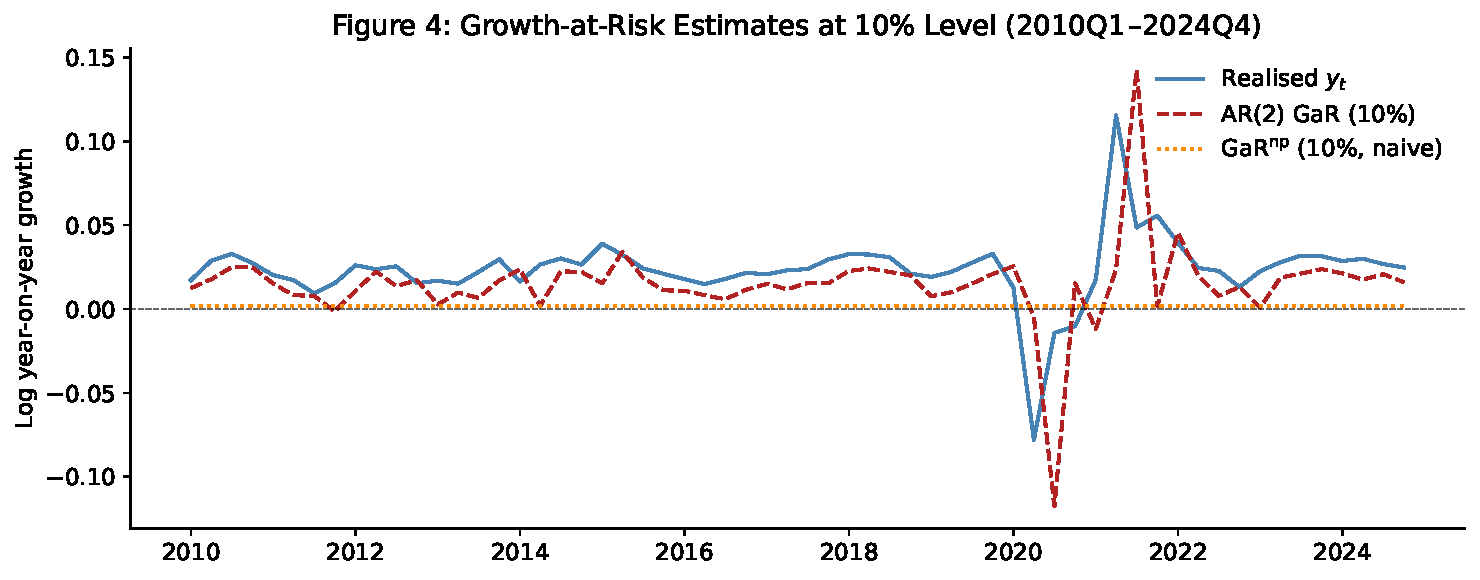
\includegraphics[width=\textwidth]{figures/fig4_gar.pdf}
    \caption{Growth-at-Risk estimates (10\% level) vs realised GDP growth, 2010Q1--2024Q4.}
    \label{fig:gar}
\end{figure}

\begin{table}[H]
    \centering
    \caption{GaR evaluation: violation rates, coverage test, and tick loss.}
    \label{tab:gar_eval}
    % \begin{table}[H]
  \centering
  \caption{GaR evaluation at 10\% level: violation rates, coverage test, and tick loss (2010Q1--2024Q4).}
  \label{tab:gar_eval}
  \begin{tabular}{lrrrr}
  \toprule
  GaR series & Violation rate p̂ & t-stat (H₀: p̂ = 0.10) & p-value & Mean tick loss \\
  \midrule
  AR(2) GaR & 0.1500 & 1.2910 & 0.1970 & 0.0046 \\
  GaR_np (naive) & 0.0500 & -1.2910 & 0.1970 & 0.0040 \\
  \bottomrule
  \end{tabular}
\end{table}

\end{table}


% ─────────────────────────────────────────────────────────────────────────────
\section{Discussion}
% ─────────────────────────────────────────────────────────────────────────────
% [1] Limitations of the Gaussian error assumption (heavy tails, COVID outlier).
% [2] Fixed parameter estimation: no recursive re-estimation over eval period.
% [3] Purely univariate: no macro/financial covariates that may predict downturns.
% [4] Parsimony vs richer models: reference Adrian et al. (2025) finding that
%     simple models need not be dominated by ML approaches.


% ─────────────────────────────────────────────────────────────────────────────
\section{Conclusion}
% ─────────────────────────────────────────────────────────────────────────────
% [1] Restate main question.
% [2] Summarise preferred model and estimation approach.
% [3] Key forecast finding (relative to naive benchmark).
% [4] Key GaR finding (coverage, tick loss vs GaR_np).
% [5] Brief outlook / limitation acknowledgement.


\end{document}